\chapter{Lernen durch Dialog}

Um einen Bezug zwischen der Serverless-Technologie und dessen Anwendung anhand eines Beispiels herzustellen, und die Evaluation der Technologie entsprechend einzuordnen, ist es sinnvoll, auch in den pädagogischen bzw. bildungswissenschaftlichen Aspekten einen Überblick zu haben. Darum geht es in diesem Kapitel.

\section{Ein Beispiel}
Für die Evaluation der Serverless-Prinzipien bedarf es eines Beispiels, welches möglichst viele typische Aspekte eines innovativen, digitalen Produkts abdeckt. Dazu gehören die Registrierung und der Login von Nutzern, öffentliche und private Informationen, dynamische und statische Daten und die damit verbundenen, regulierten Interaktionsmöglichkeiten. Der Zugang soll aus Nutzersicht durch einem beliebigen Browser und Gerät stattfinden. Eine im Rahmen des Moduls Entrepreneurship für Informatiker definierte Idee im Umfeld des E-Learnings bildet alle dieser Aspekte ab. Gleichzeitig ist die Idee, welche in den folgenden Abschnitten erläutert wird, ein interessanter Anwendungsfall, und soll einer ausführlichen Validierung in Form von Experimenten mit einem minimal funktionsfähigen Produkt (MVP)\footnote{Siehe Abschnitt \ref{sub:mvp}} unterzogen werden.

\section{Der Lehrauftrag}
\label{sec:teach}
Lehrer und Professoren haben die Aufgabe, Wissen zu vermitteln. Dafür gibt es bereits viele digitale Werkzeuge ganz unterschiedlicher Art, von denen bereits einige gut skalieren. Ein Beispiel ist Moodle\footnote{\url{https://moodle.org/}}, in dem Kurse angelegt und mit Inhalten, Referenzen, Videos, Abgabemöglichkeiten und Aufgaben gefüllt werden können. In den Moodle-Kursen sind in der Regel Menschen registriert, die sich außerhalb der Plattform im Rahmen des Kurses regelmäßig treffen, wie beispielsweise Schulklassen oder Hochschulkurse. Dazu passend sind die Nutzer auf der Plattform weder anonym noch pseudonym, sondern agiert mit seinem echten Namen. Ein weiteres Beispiel ist YouTube, welches ebenfalls für den Zweck der Wissensvermittlung genutzt werden kann. Die Harvard University hat einige Vorlesungsreihen vollständig auf diese Plattform hochgeladen, wie beispielsweise \emph{Justice: What's the right thing to do?} von Michael Sandel, welche mit über 34 Millionen Aufrufen, mehr als 333.000 Likes und 16.000 Kommentaren\footnote{Siehe https://youtu.be/kBdfcR-8hEY} auch außerhalb der Harvard University große Beachtung finden konnte. Durch die Verwendung dieser öffentlichen Plattform skaliert die Wissensvermittlung in Richtung der Konsumenten zwar besser, der Austausch über diese Inhalte und die kollaborative Erarbeitung ist hingegen kaum abbildbar. Lehrer stehen also vor der Wahl, öffentliche oder private Werkzeuge zu benutzen, wobei sich öffentlichere Plattform durch die höhere Anonymität nur schwieriger strukturieren lassen, während weniger skalierbare Lösungen wie private Moodle Räume leichter zu strukturieren sind. Die Distribution der Struktur der Lerninhalte soll nicht bzw. nur indirekt in Lightbulb Learning abgebildet werden, daher lässt sich das Werkzeug mit anderen Werkzeugen, die genau dieses Ziel verfolgen, kombinieren.

\section{Der Evaluationsauftrag}
\label{sec:eval}
Neben der unidirektionalen Vermittlung von Wissen gehört es zum Lehrauftrag häufig auch dazu, bei den Schülern oder Studenten zu beurteilen, ob das Gelernte tatsächlich verstanden wurde und angewendet werden kann. Dies wird im Folgenden als Lernevaluation bezeichnet. Hierfür nutzen Lehrer und Professoren Prüfungen, diese sind typischerweise Klausuren, oder auch alternative Leistungsnachweise in Form von Projekten, Präsentationen oder Ausarbeitungen. Diese können je nach Kontext durchaus pädagogisch wertvoller sein als reguläre, schriftliche Klausuren, gehen aber gleichzeitig mit dem Problem der fehlenden Skalierbarkeit einher. Aus diesem Grund der Praktikabilität kommt für größere Kurse häufig nur eine Klausur in Frage, welche die zunehmende Skalierbarkeit mit pädagogischer Sinnhaftigkeit bezahlt. Besonders stark ist dieser Effekt bei Multiple-Choice-Klausuren zu beobachten. Diese können neben der Variante auf Papier auch mit digitalen Werkzeugen abgebildet und automatisiert ausgewertet werden. Jedoch trainiert die Vorbereitung auf Multiple-Choice-Klausuren häufig die Fähigkeit, wiederzugeben wie die richtigen Antworten aussehen, und nicht, was deren inhaltliche Bedeutung ist \cite{Dorsch2022}. Aus Sicht eines Prüflings gestaltet sich die Optimierung auf eine solche Prüfung also nicht durch das langfristige Erlernen und Verstehen von Zusammenhängen, sondern durch das kurzfristige Auswendiglernen von Formulierungen. Hinzu kommen wahrscheinlichkeitstheoretische Effekte, insbesondere unter Einbeziehung des Ausschlussverfahrens, welche zu einer sinkenden Validität eines solchen Tests führen. Dies "verringert die Akzeptanz des Tests bzw. reduziert dessen Image im Bezug auf wiss. Seriosität und Verbindlichkeit", fasst \cite[][unter (4)]{Dorsch2022} zusammen. Die Multiple-Choice-Prüfung ist ein besonders extremes Beispiel steigender Skalierbarkeit, welche mit sinkendem pädagogischem Sinn abgegolten wird.

\section{Die Vision}
Die Vision von Lightbulb Learning ist die Erschaffung eines pädagogisch vertretbaren Lern-Evaluationssystems, welches gleichzeitig skaliert. Die Kontexte, in denen ein solchen Werkzeug eingesetzt werden könnte, sind die Schulbildung, die Hochschulbildung und Onlinekurse. Da unterschiedliche Rollen am Prozess partizipieren, sind für ein gesamtheitliches Verständnis auch die wichtigsten Perspektiven zu betrachten: Die des Professors (oder Lehrers oder Kursautors), und die des Studenten (oder Schülers oder Kursteilnehmers), welche im Folgenden jeweils austauschbar verwendet werden. Da das Lern-Evaluationssystem in unterschiedlichen Kontexten unterschiedliche Zielgruppen bedient, wird eine Festlegung auf die Begriffe eines einzigen Kontexts nicht den Anforderungen an das Systems gerecht.

\section{Zielgruppen}
\subsection{Professoren, Lehrer und Kursautoren}
Aus Sicht der Professoren soll dieses System dabei unterstützen, qualitative Evaluationen der studentischen Leistungen zu erstellen, während der Aufwand für diese Tätigkeit pro Student möglichst gering gehalten werden soll, um möglichst viele Studenten bewerten zu können und damit die Skalierbarkeit aufrecht zu erhalten. Im akademischen Kontext ist das Wertversprechen einer Lösung, welche diese Anforderungen erfüllt, ein Zeitgewinn für den Professor. Wendet man diese Systemanforderungen außerhalb des akademischen Kontextes an, so könnten beispielsweise Autoren von Online-Kursen dieses Werkzeug verwenden, um denjenigen Kursteilnehmern, die einen bestimmten inhaltlichen Fortschritt nachweisen können, ein entsprechendes Zertifikat ausstellen. Somit lässt sich festhalten, dass die Anforderungen an das System aus Sicht dieser Rolle vor allem Skalierbarkeit und Evaluationsqualität sind.

\subsection{Studenten, Schüler und Kursteilnehmer}
In diesem Abschnitt soll die Perspektive des Lerners eingenommen werden, um dessen Prioritäten, Bedürfnisse und Wünsche zu beleuchten. So ist beispielsweise im klassischen akademischen Kontext die studentische Perspektive auf die Frage der Bewertung eine völlig andere als die des Professors. Es ist besonders wichtig, fair und valide beurteilt zu werden, und in einem System zu lernen, indem langfristiges Lernen\footnote{als Gegensatz zum kurzfristigen Auswendiglernen} belohnt wird. Die Fairness ist ein Aspekt, der vor allem aus dem sozialen Umfeld der Studenten entsteht und nicht in jedem Kontext die gleiche Bedeutung hat, da etwa für Onlinekurse möglicherweise kein Bezug zu anderen Teilnehmern besteht, welche einen direkten Vergleich überhaupt ermöglichen würden. Für diese Fälle ist der Begriff der Fairness eher im Sinne der Nachvollziehbarkeit zu deuten. Die Validität rückt aus der Sicht der Lerners häufig erst nach der Prüfung in den Vordergrund: Hat jemand eine Prüfung bestanden und eine entsprechende Note dafür erhalten, so ist es aus Sicht des Absolventen von zentraler Bedeutung, dass das Bestehen eine mit Aufwand und Fähigkeiten erarbeitete, nicht inflationäre Leistung ist, und auch von der Außenwelt als solche wahrgenommen wird. Im Kontext eines Onlinekurses spielt die Bedeutung der Validität eine besondere Rolle, da sie besonders gefährdet ist. Liegen beispielsweise die Antworten auf einen Fragekatalog im Internet bereits öffentlich vor, so kann die Validität der Leistung der Beantwortung dieser Fragen selbst dann in Mitleidenschaft gezogen werden, wenn die fertigen Antworten nicht verwendet wurden, da dies durch das unkontrollierbare Umfeld des Prüflings nicht ausgeschlossen werden kann. Zusammenfassend lässt sich sagen, das aus der Perspektive der Lerner insbesondere die Fairness, die Validität und der Rahmen, der langfristiges Lernen fördert, von zentraler Bedeutung sind.

\section{Die Idee}
\label{sec:idea}
Die beschrieben Anforderungen sollen mittels eines innovativen digitalen Werkzeugs adressiert und umgesetzt werden. Der Kern für die Umsetzung der beschriebenen Anforderungen ist das Crowdsourcing bzw. die Schwarmauslagerung. Studenten erhalten den Auftrag, selbst Fragen zu formulieren, die Fragen der anderen Studenten zu diskutieren und zu beantworten, und sich gegenseitig Feedback zu geben. Dabei ist jede Facette dieser Leistung, also jede Form der Interaktion, ein Teil der Gesamtleistung, was eine pädagogisch vertretbare Form der gegenseitigen Wissensvermittlung und individuellen Wissensaufnahme ermöglicht. Zeitgleich ermöglicht sie detaillierte Einblicke in die Entwicklung des Wissensstands eines Studenten über einen längeren Zeitraum, beispielsweise über das gesamte Semester. Ein Professor kann die Übersicht sämtlicher Leistungen eines Studenten in chronologischer Reihenfolge zu jeder Zeit einsehen, was einen guten Eindruck über das Leistungsniveau des Studenten vermittelt. So ist nicht nur frühes Feedback in Richtung des Studenten und die Möglichkeit der Verbesserung fehlender Leistung möglich, sondern wird auch dem Professor widergespiegelt, auf welchem Niveau der Kurs als Ganzes sich befindet. Dies kann (und sollte) Auswirkungen auf die Lehre haben, um dem in Abschnitt \ref{sec:teach} bereits beschriebenen Lehrauftrag möglichst gut nachzukommen. Auch für den Kontext der Onlinekurse greifen die gleichen Mechanismen. Durch die schnelle Bewertbarkeit kann ein Kursautor einen interaktiveren Umgang mit seinen Kursteilnehmern haben und diese individuell bewerten, was vorher nicht möglich gewesen wäre. Weshalb die Interaktion der Prüflinge untereinander einen guten Überblick über das Leistungsniveau der partizipierenden Individuen gibt, wird in den folgenden Kapiteln beschrieben.

\subsection{Offene Fragen}
Insbesondere die Fähigkeit gute, originelle und offene Fragen zu einem bestimmten Themenbereich zu stellen, bezeugt sehr stark die Tiefe des Verständnisses, welche der Verfasser der Frage zu dem Zeitpunkt hat. Diese Aussage stützt sich auf die Begründung, dass beim Erstellen einer Frage immer der Kontext, der Problemraum und die Relevanz der Frage definiert werden muss, während eine Antwort typischerweise diesen Kontext lediglich aufgreift. Ein einfaches Beispiel aus dem Themenbereich des Quantencomputings könnte lauten: „Was sind die wesentlichen Unterschiede zwischen einem Qubit und einem normalen Bit?”. Um eine solche Frage zu stellen, muss dem Fragesteller klar sein, dass es einen Unterschied gibt, und die Frage nach dem Unterschied aus seiner Sicht eine bedeutende Rolle für das Verständnis von Qubits, oder im weiteren Sinne von Quantencomputing, spielt. Der Antwortgeber hingegen bekommt den Problemraum vorgelegt, und muss innerhalb dessen lediglich eine Antwort formulieren. Gleichzeitig ermöglichen gute Fragen eine qualitativ hochwertige Diskussion durch die Beantwortung - der wiederum einen Mehrwert für alle Beteiligten darstellt. Somit kann nicht nur Verständnis und dessen Kontext durch eine gute Frage ausgedrückt werden, sondern werden auch die Fähigkeiten der Kommunikation, insbesondere der Moderation, trainiert, welche in der modernen Arbeitswelt von zentraler Bedeutung sind.

\subsection{Antworten auf offene Fragen}
Die Funktion des Arbeitsauftrags einer Antwort ist naheliegend: es wird der Umgang mit den Werkzeugen der Problemlösung, beispielsweise der Internetrecherche oder Lernvideos, sowie der Adaption von theoretischem Wissen auf einen konkreten Kontext trainiert und bewertet. Neben dem Leistungsnachweis, Fragen korrekt und präzise beantworten zu können, greifen noch weitere Mechanismen, wie die Externalisierung im Sinne des SECI-Modells\footnote{SECI = Sozialisation, Externalisierung, Kombination, Internalisierung} \cite{Nonaka1997}. Damit ist gemeint, dass implizites Wissen zu explizitem Wissen transformiert wird, indem es formuliert wird. Im darauffolgenden Schritt der Kombination im Rahmen der Diskussion der Frage bzw. einer bestimmten Antwort kann dieses von anderen Studenten durch die Internalisierung wiederum zu implizitem Wissen und daher angewendet werden. Gleichzeitig wirkt die Antwort als Feedback an den Fragesteller. Beispielsweise sind Ein-Wort-Antworten, welche eine Frage korrekt und präzise beantworten, gute Hinweise darauf, dass die Qualität bzw. die Offenheit dieser Frage eher gering war. Ist eine Frage zu unklar formuliert, so könnten Antworten von unterschiedlichen Studenten diese stark unterschiedlich beantworten. Erhält eine Frage hingegen mehrere, ausführliche Antworten, welche im Laufe der Zeit mehrfach korrigiert und präzisiert werden, so ist die Wahrscheinlichkeit, dass es sich um eine gute Frage handelt, deutlich erhöht. Wurde eine Antwort einmal gegeben, so muss diese nicht endgültig sein.

\subsection{Feedback}
Erhält der Verfasser einer Antwort Feedback darauf, so kann er seine Antwort auf die Frage im Sinne der Korrektur und Präzisierung verbessern. Gleichzeitig ist auch der Prozess des gegenseitigen Feedback-Gebens für den Verfasser des Feedbacks hilfreich. Der Empfänger des Feedbacks erhält die Gelegenheit, Aspekte in seine Antwort einzubeziehen, welche er vorher nicht in Erwägung gezogen hatte, oder auch klare Fehler zu korrigieren. Da er gleichzeitig aber auch im vollen Bewusstsein dessen ist, dass der Feedback-Geber selbst nicht zwangsläufig ein Experte für den behandelten Themenbereich sein muss, muss er ein eigenes Urteil für die Einordnung und den Umgang mit dem Feedback bilden. Durch die Augenhöhe des Feedbacks steht der Verbesserungsprozess eher im Vordergrund als die Bewertung der Leistung, denn diese wird von einer anderen Person als vom Feedbackgeber durchgeführt. Daraus geht hervor, dass sich der Fokus mehr auf die Verbesserung der Inhalte selbst konzentriert, und weniger auf die Einordnung des Feedbacks als Bewertung. Der Feedbackgeber trainiert seinerseits ebenfalls eine Kompetenz, welche in einem Arbeitsleben, in dem in kleinen Teams eng zusammengearbeitet wird, zunehmend wichtiger wird. So kann mit Feedback etwa nicht nur Korrekturbedarf, sondern auch Wertschätzung ausgedrückt werden. Auch Coursera, eine E-Learning-Plattform, welche in Abschnitt \ref{sub:coursera} noch genauer beschrieben wird, verwendet gegenseitiges Feedback, geht hier allerdings noch weiter und fordert die Kursteilnehmer sogar auf, sich gegenseitig eine Note zu geben \cite{Coursera2022peer}.

\subsection{Andere Typen von Lernartefakten}
Die beschriebenen offenen Fragen, deren Antworten sowie Feedback auf diese Antworten bilden nur einen kleinen Teil der Formen ab, die ein Lernartefakt annehmen kann. Einige weitere Beispiele wären Programmiercode, Mathematikaufgaben bzw. deren Lösungen, Visualisierungen wie Graphen, Skizzen oder Pläne, Aufsätze, Bilder, Videos oder Tonaufnahmen. Technisch gesehen wäre es möglich, diese ebenfalls in die Entwicklung von Lightbulb Learning einzubeziehen. Dennoch wird für den Kontext dieser Thesis der Fokus auf den Aufgabentyp \emph{offene Frage} gelegt, da dieser einen Kompromiss zwischen der Einfachheit der Umsetzung, was eine schnelle Validierung durch Nutzer ermöglicht, und der Breite der Anwendungsmöglichkeiten darstellt.

\subsection{Crowdsourcing}
Lightbulb Learning beinhaltet selbst keine Intelligenz in der Hinsicht der Einordnung, Strukturierung oder Filterung von Inhalten, sondern stellt lediglich ein Werkzeug für Kurse bereit, dies kollaborativ erledigen können. Es stellt sich allerdings die Frage, ob das System durch nicht-technische Angriffe wie Absprachen manipulierbar ist. Ein mögliches Szenario für einen solchen Versuch wäre die Clusterbildung. Damit ist gemeint, dass Leute sich eher an den Teilen des Diskussion beteiligen, die von ihren jeweiligen Bekannten dominiert werden. Über Kommunikationskanäle außerhalb von Lightbulb Learning könnte sinngemäß etwa vereinbart werden, dass sich jeder ein paar Fragen überlegt, den anderen die Antworten schickt und diese die Antworten, ohne dabei das entsprechende Verständnis aufzubauen, nur noch in das System eintragen. Das ist prinzipiell möglich, aber für die Erlangung einer guten Bewertung nicht sinnvoll und leicht zu entdecken. Inhaltlich gleiche Antworten oder gleiche Formulierung auf eine Frage können als Hinweise aufgefasst werden. Zusätzlich wäre es auch möglich, eine Analyse des Interaktionsgraphen durchzuführen, welche die Clusterbildung erkennt und den Professor auf Anomalien hinweist. Insbesondere in Hinsicht der Nutzung des Like-Features für Fragen und Antworten hätte eine solche Analyse eine besondere Aussagekraft. Dabei ist zu jedoch auch zu beachten, dass Clusterbildung nicht unbedingt ein Missbrauchsversuch ist, sondern auch schlicht Überlappungen von Interessensbereichen beschreiben kann. Insbesondere können solche Cluster auch als Lerngruppen begriffen werden, welche durch den Austausch über die Inhalte eines Kurses aktiv dazu beitragen, die eigene Lernqualität zu erhöhen.

\subsection{Formatives und summatives Assessment}
Bei Prüfungen unterschiedlicher Art, wie sie heutzutage im akademischen Kontext gängig sind, handelt es sich in den meisten Fällen um summatives Assessment. Damit ist gemeint, dass beispielsweise durch eine schriftliche oder mündliche Klausur am Ende eines Semesters eine Wissensabfrage mit dem Ziel der Lernevaluation für den gesamten Zeitraum erfolgt. Formatives Assessment gibt im Gegensatz dazu über die gesamte Laufzeit des Semesters Einblicke in den aktuellen Lernstand der Studenten, so dass die Lernkurve durch individuelle Intervention korrigiert werden kann. Dieser Ansatz ist somit für den Professor deutlich aufwendiger und kann nur in kleineren Kursgrößen angewendet werden, erhöht aber sowohl die Lern- als auch die Evaluationsqualität. Eine passende Metapher für summatives Assessment ist das Foto vom Zieleinlauf des NYC Marathons in Abbildung \ref{fig:mara}. Hier wird die gesamte Leistung des Absolvierens eines Marathons auf eine einzige, sehr eindimensionale Metrik vereinfacht. Auch wenn dieser Ansatz seine Daseinsberechtigung hat, nämlich in der Frage, wer am schnellsten 42,195 Kilometer zufuß zurücklegen kann, fallen Aspekte wie die Körpergröße, das Gewicht, Verletzungen auf den letzten Kilometern oder die Qualität der Ausrüstung überhaupt nicht ins Gewicht.

\begin{figure}[H]
    \centering
    
\includegraphics[width = .5\textwidth]{images/nycm.jpeg}
    \caption{Zieleinlauf des NYC Marathons 2018
        \newline
        Quelle: \url{https://www.nyrr.org/tcsnycmarathon/getinspired/photos-and-stories/marathon-goals-virtual-training}
    }
    \label{fig:mara}
\end{figure}

\noindent Lightbulb Learning verfolgt das Ziel, eine Plattform für die Skalierung von formativem Assessment zu sein. In der Marathon-Metapher entspräche dies einem vollständigen Streckenprotokoll der Läufer mit mehreren Checkpoints, wie in Abbildung \ref{fig:graph} dargestellt. Im übertragenen Sinne sind dabei mehr unterschiedliche Messpunkte und die Messung über einen längeren Zeitraum entscheidend.

\begin{figure}[H]
    \centering
    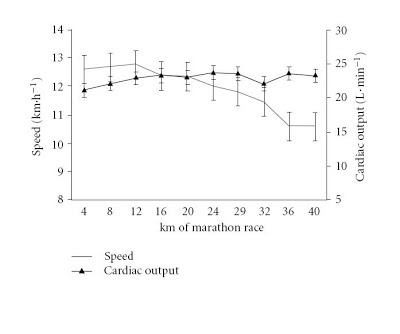
\includegraphics[width = .7\textwidth]{images/mrep.png}
    \caption{Streckenprotokoll über Londoner Marathon
        \newline
        Quelle: \url{https://ultrastu.blogspot.com/2013/05/the-negative-split-fallacy-part-2.html}
    }
    \label{fig:graph}
\end{figure}